\documentclass[11pt, a4paper]{article}

% Deutsche Sprachanpassungen und Zeichenkodierung
\usepackage[utf8]{inputenc}
\usepackage[T1]{fontenc}
\usepackage[ngerman]{babel}
\usepackage{csquotes} % Für korrekte Anführungszeichen mit biblatex

% Seitenlayout
\usepackage[a4paper, margin=2.5cm]{geometry}

% Mathematische Symbole
\usepackage{amsmath}

% Für Bilder
\usepackage{graphicx} 
\usepackage{float} % Für genaue Positionierung von Bildern mit H

% Für Code-Listings
\usepackage{listings}
\usepackage{xcolor} % Für farbigen Code

% Für Literaturverzeichnis
\usepackage{biblatex}
\addbibresource{literatur.bib} % Erstellen Sie diese Datei für Ihre Quellen

\lstdefinestyle{pythonstyle}{
    language=Python,
    basicstyle=\ttfamily\small,
    keywordstyle=\color{blue},
    stringstyle=\color{red!60!black},
    commentstyle=\color{green!50!black}\itshape,
    morecomment=[l][\color{magenta}]{\#},
    showstringspaces=false,
    tabsize=4,
    breaklines=true, % Zeilenumbruch bei langen Zeilen
    breakatwhitespace=true, % Umbruch nur bei Leerzeichen
    captionpos=b % Position der Caption (unten)
}
\lstset{style=pythonstyle}


% --- Dokumentinformationen ---
\title{Bericht zu Übungsblatt 1: \\ Primzahlen und Grundlagen der Bildverarbeitung mit OpenCV}
\author{Nik Tykhomyrov \and Jonas Pardeyke}
\date{\today} % Setzt das aktuelle Datum


\begin{document}

\maketitle

\tableofcontents
\newpage

% --- 1. Einleitung ---
\section{Einleitung}

\subsection{Thema und Kontext}
Diese Arbeit dokumentiert die Bearbeitung ausgewählter Aufgaben des Übungsblattes 1 im Modul BV1 (Bildverarbeitung 1). Der Fokus liegt dabei auf zwei Kernbereichen: der algorithmischen Generierung von Primzahlen und den grundlegenden Operationen der digitalen Bildverarbeitung mittels der Programmiersprache Python und der Bibliothek OpenCV. Die Aufgaben dienen als Einstieg in die praktische Arbeit mit Entwicklungsumgebungen und relevanten Bibliotheken für die Bildverarbeitung \cite{opencv}.

\subsection{Ziele}
Das primäre Ziel dieser Arbeit ist die praktische Umsetzung und Dokumentation der Lösungen für die Aufgaben 3 bis 7 des Übungsblattes \cite{uebungsblatt}. Dies umfasst:
\begin{itemize}
    \item Die Implementierung eines Primzahlengenerators unter Verwendung einer selbstdefinierten Funktion zur Primzahlprüfung.
    \item Das Einlesen, Anzeigen, Speichern und erneute Laden eines digitalen Bildes unter Verwendung von OpenCV.
    \item Die Untersuchung der Auswirkungen verlustbehafteter Kompression (JPEG) durch den Vergleich des Originalbildes mit seiner komprimierten Version mittels einer geeigneten Punktoperation.
    \item Die Erklärung der zugrundeliegenden Konzepte und der verwendeten Werkzeuge.
\end{itemize}
Das übergeordnete Ziel ist es, grundlegende Programmierkenntnisse in Python zu festigen und erste Erfahrungen im Umgang mit digitalen Bildern und der OpenCV-Bibliothek zu sammeln.

\subsection{Relevanz}
Die in dieser Arbeit behandelten Themen sind von grundlegender Bedeutung. Primzahlen spielen eine wichtige Rolle in der Kryptographie und der theoretischen Informatik. Die digitale Bildverarbeitung ist ein omnipräsentes Feld mit Anwendungen von der Medizintechnik über die industrielle Qualitätskontrolle bis hin zur Unterhaltungselektronik und autonomen Systemen. Das Verständnis von Bildformaten, Kompressionsverfahren wie JPEG und grundlegenden Analyseoperationen ist essenziell für weiterführende Arbeiten in diesem Bereich. Die Fähigkeit, Bilder programmgesteuert zu laden, zu manipulieren und zu speichern, ist eine Kernkompetenz.

\subsection{Aktueller Stand und Grundlagen}
\subsubsection{Primzahlengenerierung}
Die Bestimmung von Primzahlen ist ein klassisches Problem der Zahlentheorie. Effiziente Algorithmen sind für viele Anwendungen entscheidend. Ein grundlegender Ansatz ist die Probedivision, die hier mit einer Optimierung (Prüfung nur bis zur Quadratwurzel) implementiert wird. Für sehr große Zahlen existieren wesentlich komplexere probabilistische (z.B. Miller-Rabin) und deterministische Tests.

\subsubsection{Bildverarbeitung mit Python und OpenCV}
Python hat sich zusammen mit Bibliotheken wie OpenCV (Open Source Computer Vision Library) und NumPy (Numerical Python) als Standardwerkzeug in der Bildverarbeitung etabliert. OpenCV bietet eine breite Palette von Funktionen für Bild- und Videoanalyse, während NumPy die effiziente Handhabung von Bilddaten als mehrdimensionale Arrays ermöglicht.

\subsubsection{Digitale Bilder und Kompression}
Ein digitales Bild wird typischerweise als Raster von Pixeln repräsentiert, wobei jeder Pixel einen Farb- oder Helligkeitswert speichert (z.B. über RGB-Kanäle). Bilddateiformate unterscheiden sich in ihrer Speicherung und Kompression. JPEG (Joint Photographic Experts Group) ist ein weit verbreitetes \textit{verlustbehaftetes} Kompressionsverfahren, optimiert für fotografische Bilder. Es reduziert die Dateigröße signifikant, indem es Informationen entfernt, die für das menschliche Auge oft schwer wahrnehmbar sind. Dies führt jedoch zu irreversiblen Qualitätsverlusten. Im Gegensatz dazu stehen \textit{verlustfreie} Formate wie PNG, die eine exakte Rekonstruktion des Originalbildes ermöglichen, aber meist weniger Speicherplatz sparen.

\subsubsection{Punktoperationen}
Eine Punktoperation in der Bildverarbeitung ist eine Transformation, bei der der neue Wert eines Pixels ausschließlich von seinem ursprünglichen Wert abhängt, unabhängig von den Werten benachbarter Pixel. Beispiele sind Helligkeits-/Kontrastanpassung oder die Berechnung der Differenz zwischen zwei Bildern an derselben Pixelposition.

\subsection{Aufbau der Arbeit}
Diese Arbeit gliedert sich wie folgt: Nach dieser Einleitung folgt der \textbf{Hauptteil}, welcher die verwendeten Werkzeuge und grundlegenden Konzepte kurz erläutert. Anschließend wird die Implementierung des Primzahlengenerators (Aufgabe 3) beschrieben, inklusive der mathematischen Optimierung. Danach werden die Schritte zur Bildverarbeitung (Aufgaben 4-7) detailliert: das Laden und Speichern des Bildes, die Anwendung der JPEG-Kompression und die Analyse der Unterschiede mittels einer Punktoperation. Der Hauptteil schließt mit der Darstellung und Diskussion der Ergebnisse. Die Arbeit endet mit einer \textbf{Zusammenfassung und einem Ausblick}, in der die Ergebnisse rekapituliert, die Zielerreichung bewertet und mögliche weiterführende Schritte aufgezeigt werden.


% --- 2. Hauptteil ---
\section{Hauptteil}

\subsection{Verwendete Werkzeuge und Grundlagen}
Zur Lösung der Aufgaben wurde die Programmiersprache \textbf{Python} (Version 3.x) verwendet. Die wesentlichen externen Bibliotheken sind:
\begin{itemize}
    \item \textbf{OpenCV (\texttt{cv2})}: Eine umfassende Bibliothek für Computer Vision und Bildverarbeitung. Sie wurde hier für das Einlesen (\texttt{cv2.imread}), Anzeigen (\texttt{cv2.imshow} bzw. alternative Darstellung mit Matplotlib), Speichern (\texttt{cv2.imwrite}), die Berechnung der absoluten Differenz (\texttt{cv2.absdiff}) und die Skalierung von Bilddaten (\texttt{cv2.convertScaleAbs}) genutzt.
    \item \textbf{NumPy (\texttt{numpy})}: Eine fundamentale Bibliothek für numerische Berechnungen in Python. OpenCV repräsentiert Bilder als NumPy-Arrays, was effiziente pixelweise Operationen und statistische Auswertungen (z.B. \texttt{numpy.mean}, \texttt{numpy.max}) ermöglicht.
    \item \textbf{Matplotlib (\texttt{matplotlib.pyplot})}: Wurde optional zur Darstellung der Bilder innerhalb der Jupyter-Notebook-Umgebung verwendet, da \texttt{cv2.imshow} dort nicht immer zuverlässig funktioniert.
\end{itemize}

Wie in der Einleitung erwähnt, ist eine \textbf{Punktoperation} eine Bildtransformation, bei der jeder Ausgabepixelwert $g(x, y)$ nur vom Eingabepixelwert an derselben Position $f(x, y)$ abhängt: $g(x, y) = T(f(x, y))$. Die hier verwendete Differenzbildung zwischen zwei Bildern $I_1$ und $I_2$, $D(x, y) = |I_1(x, y) - I_2(x, y)|$, ist ebenfalls eine Punktoperation, da jeder Differenzpixel nur von den Werten der Eingangsbilder an der korrespondierenden $(x, y)$-Position abhängt.

\subsection{Aufgabe 3: Primzahlengenerator}
Ziel dieser Aufgabe war es, die ersten $n$ Primzahlen zu generieren, wobei die Prüfung auf Primalität in einer eigenen Funktion erfolgen sollte \cite{uebungsblatt}.

\subsubsection{Implementierung der Primzahlprüfung}
Eine Zahl $p > 1$ ist eine Primzahl, wenn sie nur durch 1 und sich selbst ohne Rest teilbar ist. Die Funktion \texttt{is\_prime} prüft dies mittels Probedivision.
\begin{lstlisting}[caption={Python-Funktion zur Prüfung auf Primalität}, label=lst:is_prime]
def is_prime(number):
    if number <= 1:
        return False
    # Prf {\"u}e Teiler nur bis zur Quadratwurzel der Zahl
    # int(number**0.5) + 1 stellt sicher, dass die Obergrenze korrekt ist
    for i in range(2, int(number**0.5) + 1):
        if number % i == 0: # Wenn teilbar, dann keine Primzahl
            return False
    return True # Keine Teiler gefunden (au{\ss}er 1 und sich selbst)
\end{lstlisting}
Die entscheidende Optimierung liegt in der oberen Grenze der Schleife: \texttt{int(number**0.5) + 1}. Mathematisch gilt: Wenn eine Zahl \texttt{number} zusammengesetzt ist (d.h. keine Primzahl), dann hat sie mindestens einen Teiler $d$ mit $d \leq \sqrt{\text{number}}$. Gäbe es nämlich keinen solchen Teiler, müssten alle Teiler größer als $\sqrt{\text{number}}$ sein. Wenn man zwei solche Teiler multipliziert, wäre das Produkt größer als $\text{number}$, was ein Widerspruch ist. Daher genügt es, Teiler bis zur Quadratwurzel von \texttt{number} zu prüfen ($\sqrt{\text{number}}$ entspricht \texttt{number**0.5}). Dies reduziert den Rechenaufwand erheblich gegenüber einer Prüfung bis \texttt{number - 1}.

\subsubsection{Implementierung des Generators}
Die Funktion \texttt{primeNumberGenerator} nutzt \texttt{is\_prime}, um sequenziell Zahlen zu testen und die ersten $n$ gefundenen Primzahlen in einer Liste zu sammeln.
\begin{lstlisting}[caption={Python-Funktion zur Generierung der ersten n Primzahlen}, label=lst:prime_gen]
def primeNumberGenerator(n):
    primes = []
    number = 2 # Erste zu pr {\"u}fende Zahl
    while len(primes) < n:
        if is_prime(number):
            primes.append(number)
        number += 1
    return primes
\end{lstlisting}

\subsubsection{Ergebnis}
Für $n=10$ liefert der Generator die korrekte Liste der ersten 10 Primzahlen: \texttt{[2, 3, 5, 7, 11, 13, 17, 19, 23, 29]}.

\subsection{Aufgaben 4-7: Bildverarbeitung und Kompressionsanalyse}
Diese Aufgabenkette befasst sich mit dem Laden eines Bildes, dessen Speicherung im verlustbehafteten JPEG-Format und der anschließenden Analyse der durch die Kompression entstandenen Unterschiede zum Original.

\subsubsection{Vorgehen}
Das Vorgehen folgte direkt den Aufgabenstellungen:
\begin{enumerate}
    \item \textbf{Laden und Anzeigen (Aufgabe 4):} Das Bild \texttt{Set01.jpg} wurde mittels \texttt{cv2.imread} geladen und zur Kontrolle angezeigt. Das geladene Bild wird als $I$ bezeichnet.
    \item \textbf{Komprimiertes Speichern (Aufgabe 5):} Das Bild $I$ wurde mit \texttt{cv2.imwrite} als \texttt{Set01\_compressed.jpg} gespeichert. Dabei wurde das JPEG-Format mit einem Qualitätsparameter von 50 (auf einer Skala von 0-100) gewählt. Eine niedrigere Qualität bedeutet höhere Kompression und potenziell größere sichtbare Artefakte.
    \item \textbf{Erneutes Laden (Aufgabe 6):} Das komprimierte Bild \texttt{Set01\_compressed.jpg} wurde mit \texttt{cv2.imread} geladen und als $I_L$ bezeichnet.
    \item \textbf{Differenzanalyse (Aufgabe 7):} Die Unterschiede zwischen dem Original $I$ und dem geladenen komprimierten Bild $I_L$ wurden mittels einer Punktoperation berechnet und visualisiert.
\end{enumerate}

\subsubsection{Implementierungsdetails}
\paragraph{Laden und Speichern:}
Das Laden erfolgt über \texttt{img = cv2.imread('filename.jpg')}. Das Speichern als JPEG mit Qualitätsstufe 50 wird realisiert durch:
\begin{lstlisting}[caption={Speichern eines Bildes als JPEG mit Qualitätsstufe 50}]
quality = 50
cv2.imwrite('Set01_compressed.jpg', imgGlobal, 
            [cv2.IMWRITE_JPEG_QUALITY, quality])
\end{lstlisting}
Hier ist \texttt{imgGlobal} die Variable, die das (Original-)Bild als NumPy-Array enthält.

\paragraph{Differenzberechnung und Visualisierung:}
Um die Unterschiede zwischen $I$ (\texttt{imgGlobal}) und $I_L$ (\texttt{imgCompressed}) sichtbar zu machen, wurde die absolute Differenz berechnet und anschließend verstärkt.
\begin{lstlisting}[caption={Berechnung und Verstärkung des Differenzbildes}]
# Berechne den absoluten Unterschied pro Pixel
# D(x, y) = |I(x, y) - I_L(x, y)|
diff = cv2.absdiff(imgGlobal, imgCompressed)

# Verst {\"a}rke die Unterschiede f {\"u}r bessere Sichtbarkeit
# D_enhanced(x, y) = saturate(alpha * D(x, y) + beta)
alpha = 10.0 # Verst {\"a}rkungsfaktor
beta = 0     # Helligkeits-Offset (hier nicht verwendet)
diff_enhanced = cv2.convertScaleAbs(diff, alpha=alpha, beta=beta) 
\end{lstlisting}
\texttt{cv2.absdiff} berechnet die absolute Differenz für jeden Pixel und jeden Farbkanal $(B, G, R)$ einzeln. Das Ergebnis \texttt{diff} ist ein Bild, bei dem Pixelwerte die Stärke der Abweichung repräsentieren. Da diese Unterschiede oft gering sind (besonders bei hoher JPEG-Qualität), werden sie mit \texttt{cv2.convertScaleAbs} verstärkt. Diese Funktion skaliert die Werte (\texttt{* alpha}) und sorgt dafür, dass das Ergebnis im gültigen Anzeigebereich für Bilder (typischerweise 0-255 für 8-Bit-Bilder) bleibt (Sättigung). Das resultierende Bild \texttt{diff\_enhanced} hebt die Bereiche hervor, in denen die Kompression die größten Änderungen verursacht hat.

\subsubsection{Ergebnisse und Diskussion}
\paragraph{Visueller Vergleich:}
Das Originalbild (Bild 1) zeigt eine Anordnung von Spielkarten mit verschiedenen geometrischen Symbolen auf einem hölzernen Untergrund. Zu sehen sind weiße Karten mit verschiedenfarbigen Symbolen wie blauen Wellenformen, roten und grünen Rauten sowie unterschiedlichen Kreisformen.

\begin{figure}[H]
    \centering
    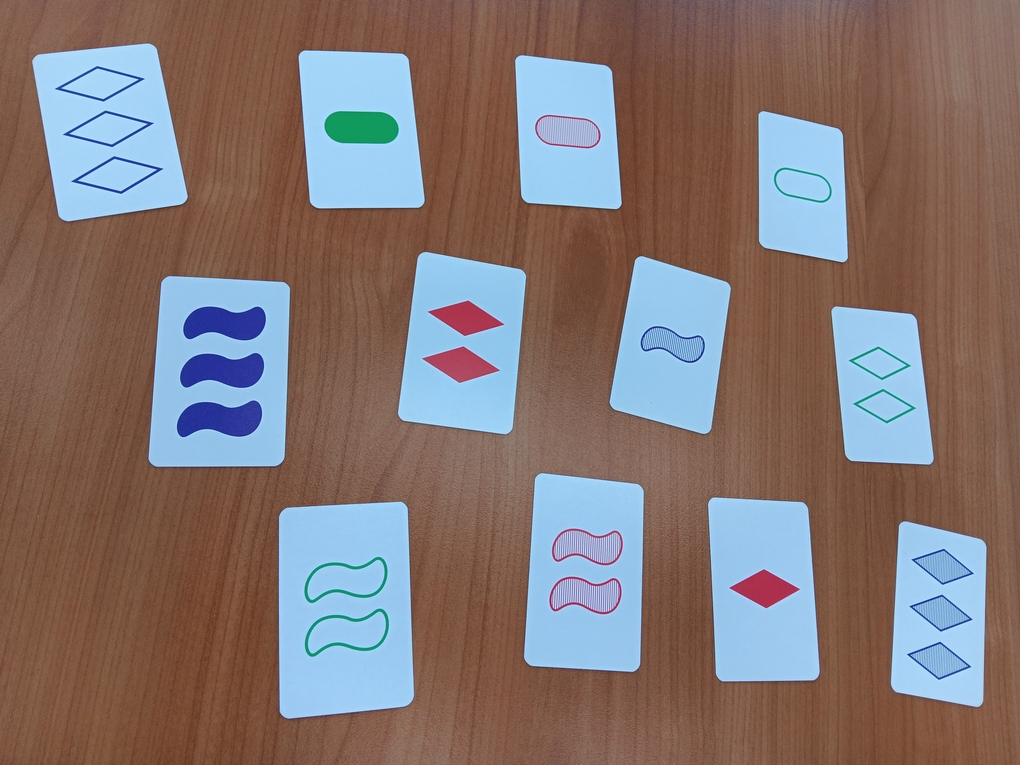
\includegraphics[width=0.8\textwidth]{Set01.jpg}
    \caption{Originalbild (Set01.jpg)}
    \label{fig:original}
\end{figure}

Das komprimierte Bild (Bild 2) erscheint auf den ersten Blick sehr ähnlich zum Original. Bei direkter visueller Betrachtung sind kaum Unterschiede erkennbar. Die Farbwiedergabe, die Konturen der Karten und der Symbole erscheinen nahezu identisch.

\begin{figure}[H]
    \centering
    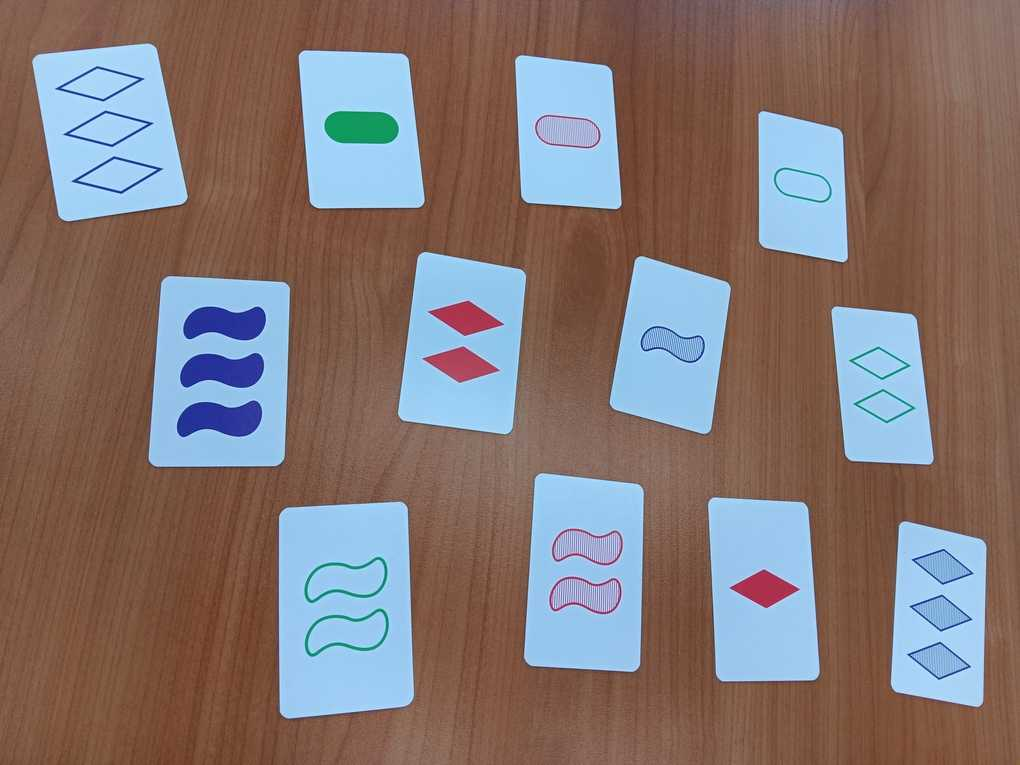
\includegraphics[width=0.8\textwidth]{Set01_compressed.jpg}
    \caption{Komprimiertes Bild (Set01\_compressed.jpg)}
    \label{fig:compressed}
\end{figure}

\paragraph{Differenzbild:}
Das verstärkte Differenzbild (Bild 3) zeigt die Auswirkungen der Kompression deutlich. Besonders auffällig sind die Konturen der Karten und der darauf abgebildeten Symbole, die sich im Differenzbild als helle Linien abzeichnen. Dies deutet darauf hin, dass die JPEG-Kompression vor allem an Kanten und Übergängen zwischen verschiedenen Farben Informationen verliert. Die farbigen Flächen innerhalb der Symbole und die homogenen Kartenflächen zeigen hingegen weniger Abweichungen.

\begin{figure}[H]
    \centering
    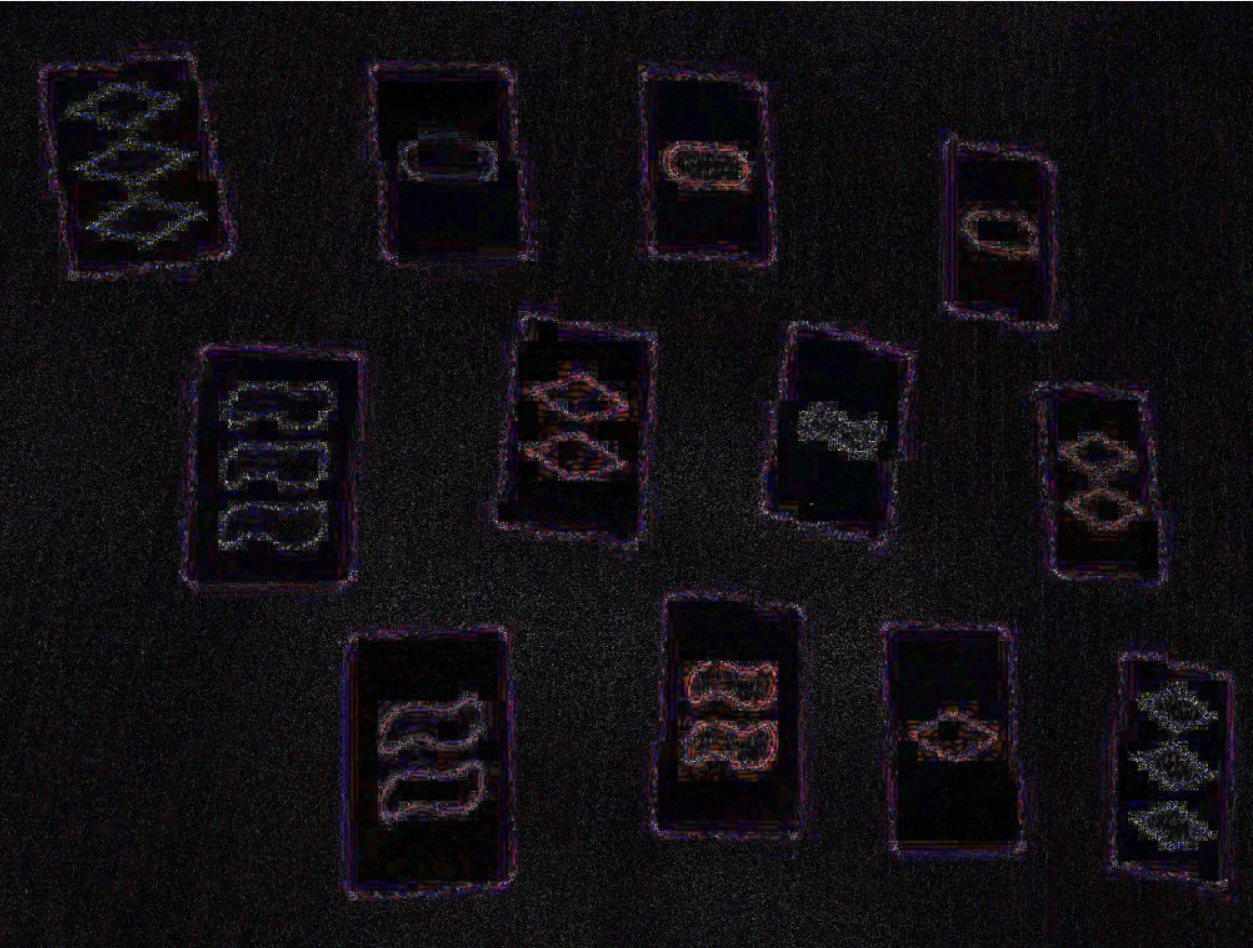
\includegraphics[width=0.8\textwidth]{diff.png}
    \caption{Verstärktes Differenzbild zwischen Original und komprimierter Version}
    \label{fig:difference}
\end{figure}

Besonders gut erkennbar sind im Differenzbild blockhafte Strukturen, die auf die 8x8-Pixel-Blöcke zurückzuführen sind, die JPEG für die Diskrete Cosinustransformation (DCT) verwendet. Diese Beobachtung ist konsistent mit der Funktionsweise von JPEG: Die Kompression basiert auf der DCT auf 8x8-Pixel-Blöcken und einer anschließenden Quantisierung, die hochfrequente Anteile (Details, Kanten) stärker reduziert als niederfrequente (grobe Strukturen).

\paragraph{Quantitative Analyse:}
Die statistische Auswertung der (unverstärkten) Differenz \texttt{diff} liefert quantitative Maße für die Abweichung:
\begin{itemize}
    \item Durchschnittlicher Unterschied pro Pixel (Mittelwert über alle Pixel und Kanäle): 3,24
    \item Maximaler Unterschied (größte Abweichung eines Pixelwertes in einem Kanal): 42
\end{itemize}
Diese Werte bestätigen, dass es messbare Unterschiede gibt, auch wenn der durchschnittliche Unterschied gering ist. Der Maximalwert zeigt, dass einzelne Pixel durchaus stärker abweichen können. Ein höherer \texttt{alpha}-Wert in \texttt{convertScaleAbs} würde diese maximalen Abweichungen im Differenzbild noch stärker hervorheben.

Die gewählte Punktoperation (\texttt{cv2.absdiff} gefolgt von \texttt{cv2.convertScaleAbs}) ist gut geeignet, um die \textit{Position} und \textit{relative Stärke} der durch verlustbehaftete Kompression eingeführten Fehler zu visualisieren.


% --- 3. Zusammenfassung und Ausblick ---
\section{Zusammenfassung und Ausblick}

\subsection{Zusammenfassung}
In dieser Arbeit wurden grundlegende Aufgaben aus den Bereichen Algorithmik und digitaler Bildverarbeitung bearbeitet. Es wurde ein funktionsfähiger Primzahlengenerator implementiert, der auf einer optimierten Primzahlprüfungsfunktion basiert. Des Weiteren wurden die Schritte zum Laden, Speichern (unter Verwendung von verlustbehafteter JPEG-Kompression mit Qualitätsstufe 50) und erneuten Laden eines digitalen Bildes mittels Python und OpenCV erfolgreich durchgeführt. Schließlich wurden die durch die JPEG-Kompression entstandenen Unterschiede zum Originalbild mittels der Punktoperation \texttt{cv2.absdiff} quantifiziert und durch Skalierung (\texttt{cv2.convertScaleAbs}) visualisiert.

\subsection{Zielerreichung}
Die zu Beginn gesetzten Ziele wurden erreicht. Die geforderten Funktionalitäten (Primzahlgenerator, Bild I/O, Kompression, Differenzbildung) wurden erfolgreich implementiert und die Ergebnisse dokumentiert. Es konnte ein grundlegendes Verständnis für die Arbeitsweise des Primzahltests, die Handhabung von Bildern in Python/OpenCV und die sichtbaren sowie messbaren Auswirkungen der JPEG-Kompression erlangt werden.

\subsection{Gelerntes}
Im Vergleich zum Stand vor der Bearbeitung wurden folgende Erkenntnisse gewonnen:
\begin{itemize}
    \item Praktische Anwendung und Optimierung von Algorithmen (Primzahltest mit $\sqrt{n}$-Grenze).
    \item Verwendung der OpenCV-Bibliothek für grundlegende Bildoperationen (I/O, arithmetische Operationen).
    \item Verständnis des Konzepts verlustbehafteter Kompression (JPEG) und dessen Konsequenzen (visuelle Artefakte, messbare Abweichungen vom Original).
    \item Anwendung von Punktoperationen zur Analyse und Visualisierung von Bildunterschieden.
    \item Bedeutung von Bibliotheken wie NumPy für die effiziente Verarbeitung von Bilddaten als Arrays.
\end{itemize}

\subsection{Empfehlungen}
Basierend auf den Ergebnissen lässt sich ableiten, dass bei der Wahl eines Bildformats und dessen Kompressionsparametern stets ein Kompromiss zwischen Dateigröße und Bildqualität eingegangen wird. Für fotografische Bilder ist JPEG oft eine gute Wahl, jedoch sollte der Qualitätsparameter bewusst gewählt werden. Für Bilder, bei denen es auf exakte Detailtreue ankommt (z.B. technische Zeichnungen, Screenshots mit Text, medizinische Bilder), sind verlustfreie Formate wie PNG vorzuziehen. Die Analyse von Differenzbildern ist ein nützliches Werkzeug zur Bewertung von Kompressionsartefakten oder anderen Bildveränderungen.

\subsection{Offene Fragen und Ausblick}
Die durchgeführten Experimente werfen weitere Fragen auf und zeigen mögliche nächste Schritte auf:
\begin{itemize}
    \item Wie verändern sich die visuellen und quantitativen Unterschiede bei \textbf{anderen JPEG-Qualitätsstufen} (z.B. 10, 90)?
    \item Wie schneiden \textbf{andere Kompressionsverfahren} (z.B. WebP, HEIC) im Vergleich zu JPEG ab?
    \item Gibt es \textbf{andere Metriken} zur Quantifizierung von Bildunterschieden, die die menschliche Wahrnehmung besser berücksichtigen (z.B. PSNR, SSIM)?
    \item Wie können die hier erlernten Grundlagen für \textbf{komplexere Bildverarbeitungsaufgaben} (z.B. Filterung, Kantendetektion, Objekterkennung) genutzt werden?
\end{itemize}
Sinnvolle nächste Schritte wären die systematische Untersuchung des Einflusses des JPEG-Qualitätsparameters, die Implementierung und der Vergleich verschiedener Differenzmetriken sowie die Anwendung der erlernten Techniken auf andere Bilder und Problemstellungen im Bereich der Bildverarbeitung.

% Bibliographie
\printbibliography

\end{document}